\section{Refund}

\begin{figure}[h!]
  \begin{sequencediagram}
    \newinst{wallet}{\shortstack{Customer wallet \\
      \\ 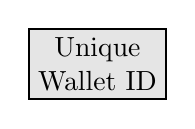
\begin{tikzpicture}
        \node [fill=gray!20,draw=black,thick,align=center] { Unique \\ Wallet ID};
      \end{tikzpicture}
    }}
    \newinst[2]{merchant}{\shortstack{Merchant \\
       \\ \begin{tikzpicture}[shape aspect=.5]
        \tikzset{every node/.style={cylinder,shape border rotate=90, draw,fill=gray!25}}
        \node at (1.5,0) {\shortstack{{{\tiny Database}}}};
       \end{tikzpicture}
    }}
    \newinst[2]{exchange}{\shortstack{Taler (exchange) \\
       \\ \begin{tikzpicture}[shape aspect=.5]
        \tikzset{every node/.style={cylinder,shape border rotate=90, draw,fill=gray!25}}
        \node at (1.5,0) {\shortstack{{{\tiny Database}}}};
       \end{tikzpicture}
    }}
    \postlevel
    \begin{callself}{merchant}{Initiate refund}{}
    \end{callself}
    \mess[0]{merchant}{{Refund offer (QR code)}}{wallet}
    \mess[0]{wallet}{Request refund}{merchant}
    \mess[0]{merchant}{Approve refund}{exchange}
    \mess[0]{exchange}{Confirm refund}{merchant}
    \mess[0]{merchant}{Return refund confirmation}{wallet}
  \end{sequencediagram}
  \caption{Refund processing when a merchant is unable to fulfill
    a contract.  Refunds must happen {\em before} the
    exchange has aggregated the original transaction for
    a bank transfer to the merchant. Furthermore, refunds
    can only go to the customer who made the original payment
    and the refund cannot exceed the amount of the original
    payment.}
  \label{fig:int:refund}
\end{figure}
